% TO-DO:
% * Actions = all possible transtions in RL
% * In RL, Q-learning is still unclear -- currently I'm using NN = transition F(x)
%   -- U(x) -> U(x') so it seems that generalization can occur in Q-space (?)
% * Structure of the turnstile is an important feature of the transition F(x)
% * Explain difference with AIXI
% * "inward" vs "outward"

\documentclass[orivec]{article}
\usepackage{graphicx}
\usepackage{amsmath}		% for "cases"
\usepackage{amsfonts}		% for frakur fonts
\usepackage{mathrsfs}		% for curly "E" error symbol
\usepackage{float}
\usepackage[most]{tcolorbox}% for wrapping example in color box
\usepackage{wrapfig}		% wrap figure beside text, used in example
\usepackage{tikz-cd}		% commutative diagrams
% \usepackage{amsfonts}
\usepackage{enumitem}       % for using (A),(B),(C) in items...
\usepackage{amssymb}		% for \multimap, \updownarrow, \bigstar
\usepackage{turnstile}		% longer turnstiles
\usepackage{sectsty}		% change section color
\usepackage{hyperref}		% refs, links become clickable
\usepackage{url}			% for urls in bibliography
\usepackage[normalem]{ulem} % underline unbroken with \uline
\usepackage[numbers,sectionbib]{natbib}% if we use \package{url} we need to use natbib style
\usepackage{verbatim}		% "comments"

%\def\chinchin{yes}          % ********** 用中文 *********
% *************** Delete when not using Chinese or colors **********************
\ifdefined\chinchin
	\usepackage{xeCJK}
	\setCJKmainfont[BoldFont=SimHei,ItalicFont=AR PL KaitiM GB]{SimSun}
\fi
\usepackage{color}
%\newcommand{\emp}[1]{\textbf{\textcolor{blue}{#1}}}
\newcommand{\emp}[1]{\textbf{#1}}

\sectionfont{\color{blue}} 
\subsectionfont{\color{blue}} 
\subsubsectionfont{\color{blue}} 
\definecolor{green}{rgb}{0,0.7,0}
\definecolor{grey}{rgb}{0.95,0.95,0.95}
\setcounter{secnumdepth}{2}			% no numbering for subsubsections

\usepackage{geometry}		% change paper size
\geometry{
  a4paper,         % or letterpaper
  textwidth=18cm,  % llncs has 12.2cm
  textheight=27cm, % llncs has 19.3cm
  heightrounded,   % integer number of lines
  hratio=1:1,      % horizontally centered
  vratio=2:3,      % not vertically centered
}
% \usepackage[fontsize=13pt]{scrextend}

\newcommand{\tikzmark}[1]{\tikz[overlay,remember picture] \node (#1) {};}

\newcommand{\vect}[1]{\boldsymbol{#1}}
\newcommand*\sigmoid{\vcenter{\hbox{
\includegraphics{sigmoid.png}}}}
\newcommand*\rectifier{\vcenter{\hbox{\includegraphics{rectifier.png}}}}
\newcommand*\KB{\vcenter{\hbox{\includegraphics{KB-symbol.png}}}}
\newcommand*\KBsmall{\vcenter{\hbox{\includegraphics{KB-symbol2.png}}}}
\newcommand*\Eye{\vcenter{\hbox{\includegraphics{../eye-symbol.png}}}}
\newcommand*\NN{\vcenter{\hbox{\includegraphics{../NN-symbol.png}}}}
\newcommand*\Graph{\vcenter{\hbox{\includegraphics{algebraic-model.png}}}}
\newcommand{\dashh}{\textemdash~}
\newcommand{\english}[1]{\mbox{\textit{#1}}}
\newcommand{\tab}{\hspace*{2cm}}

% ***** Boxed variables inside math equations
% \newcommand*{\boxedcolor}{black}
\makeatletter
% \renewcommand{\boxed}[1]{\textcolor{\boxedcolor}{%
% \fbox{\normalcolor\m@th$\displaystyle#1$}}}
% \setlength{\fboxsep}{1pt}
\renewcommand{\boxed}[1]{\fbox{\m@th$\displaystyle\scalebox{0.9}{#1}$} \,}
\makeatother

\renewcommand\labelenumi{(\theenumi)}

\overfullrule=0mm

\newsavebox{\MyName}
\savebox{\MyName}{\includegraphics[scale=0.6]{../YKY.png}}

\title{Foundation of AGI}
%\normalsize{-- a minimalist cognitive architecture combining\\
%reinforcement learning and deep learning}}
%\titlerunning{Foundation of AGI}
\author{\usebox{\MyName} (King-Yin Yan)
% \\ \footnotesize{General.Intelligence@Gmail.com}
%\and
%Ben Goertzel
%\and
%Juan Carlos Kuri Pinto
}
%\institute{General.Intelligence@Gmail.com}
\date{\today}

\begin{document}

\maketitle

\noindent
%\makebox[\linewidth]{\small \today}

\setlength{\parindent}{0em}
\setlength{\parskip}{2.8ex plus0.8ex minus0.8ex}
% \setlength{\parskip}{2.8ex}

%\begin{abstract}
%\end{abstract}

%\begin{keywords}
%reinforcement learning, control theory, deep learning, cognitive architecture
%\end{keywords}

\setcounter{section}{-1}
\section{Basic architecture}
%\label{sec:0}

首先,用一个 RNN encoder 将 自然语言 转换成 knowledge representation $\Psi$:
\begin{equation}
\vcenter{\hbox{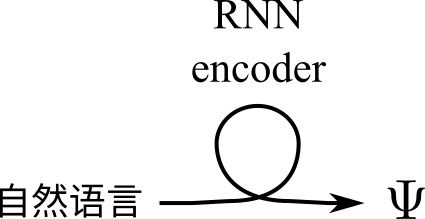
\includegraphics[scale=0.7]{AGI-foundation-1.png}}}
\end{equation}
这 \textbf{知识表述} 是人工智能中最重要的概念,它和数学上的 representation 其实是同一概念,但前者较为广义。

$\Psi$ 的特点是它可以用来做 \textbf{逻辑推导},用 $\vdash$ 符号表示:
\begin{equation}
\quad \quad \vcenter{\hbox{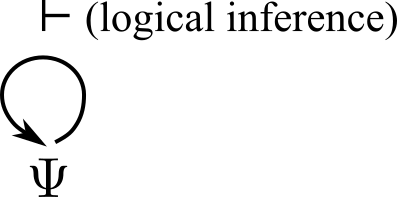
\includegraphics[scale=0.7]{AGI-foundation-2.png}}}
\end{equation}
两方面合起来就是这个基本的 architecture:
\begin{equation}
\vcenter{\hbox{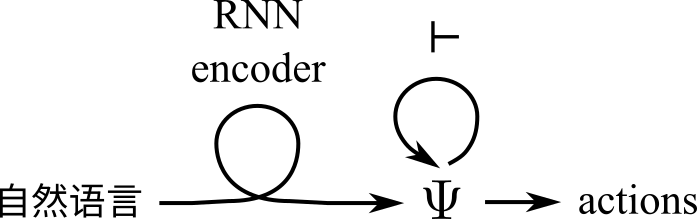
\includegraphics[scale=0.7]{AGI-foundation-3.png}}}
\end{equation}

(不排除其他读者可能有截然不同的 architectures,但这是作者最熟悉的)

整个系统是靠 deep reinforcement learning 的 Bellman update 来 进行 \textbf{学习}。 很明显,如果系统的结构复杂,会有 vanishing gradient 的危险。  系统的神经网络是庞大的(它包含所有知识),所以,有效率的学习算法,是樽颈问题。

\section{Logic}

有很多 \textbf{逻辑形式} 可以用,基本上这是个开放的问题。  在较早的 classical AI 时期,人们手动设计某些 knowledge representation schemes,但无论怎样仔细,这些 KR schemes 总会有不尽人意之处。  进入「\textbf{后结构主义}」时期,\uline{我们只是 specify abstract structure},其他细节留给 机器学习。  而这 abstract structure 的选取,似乎有很多种可能。 

以下是各种主要逻辑结构之间的关系:
\begin{equation}
\vcenter{\hbox{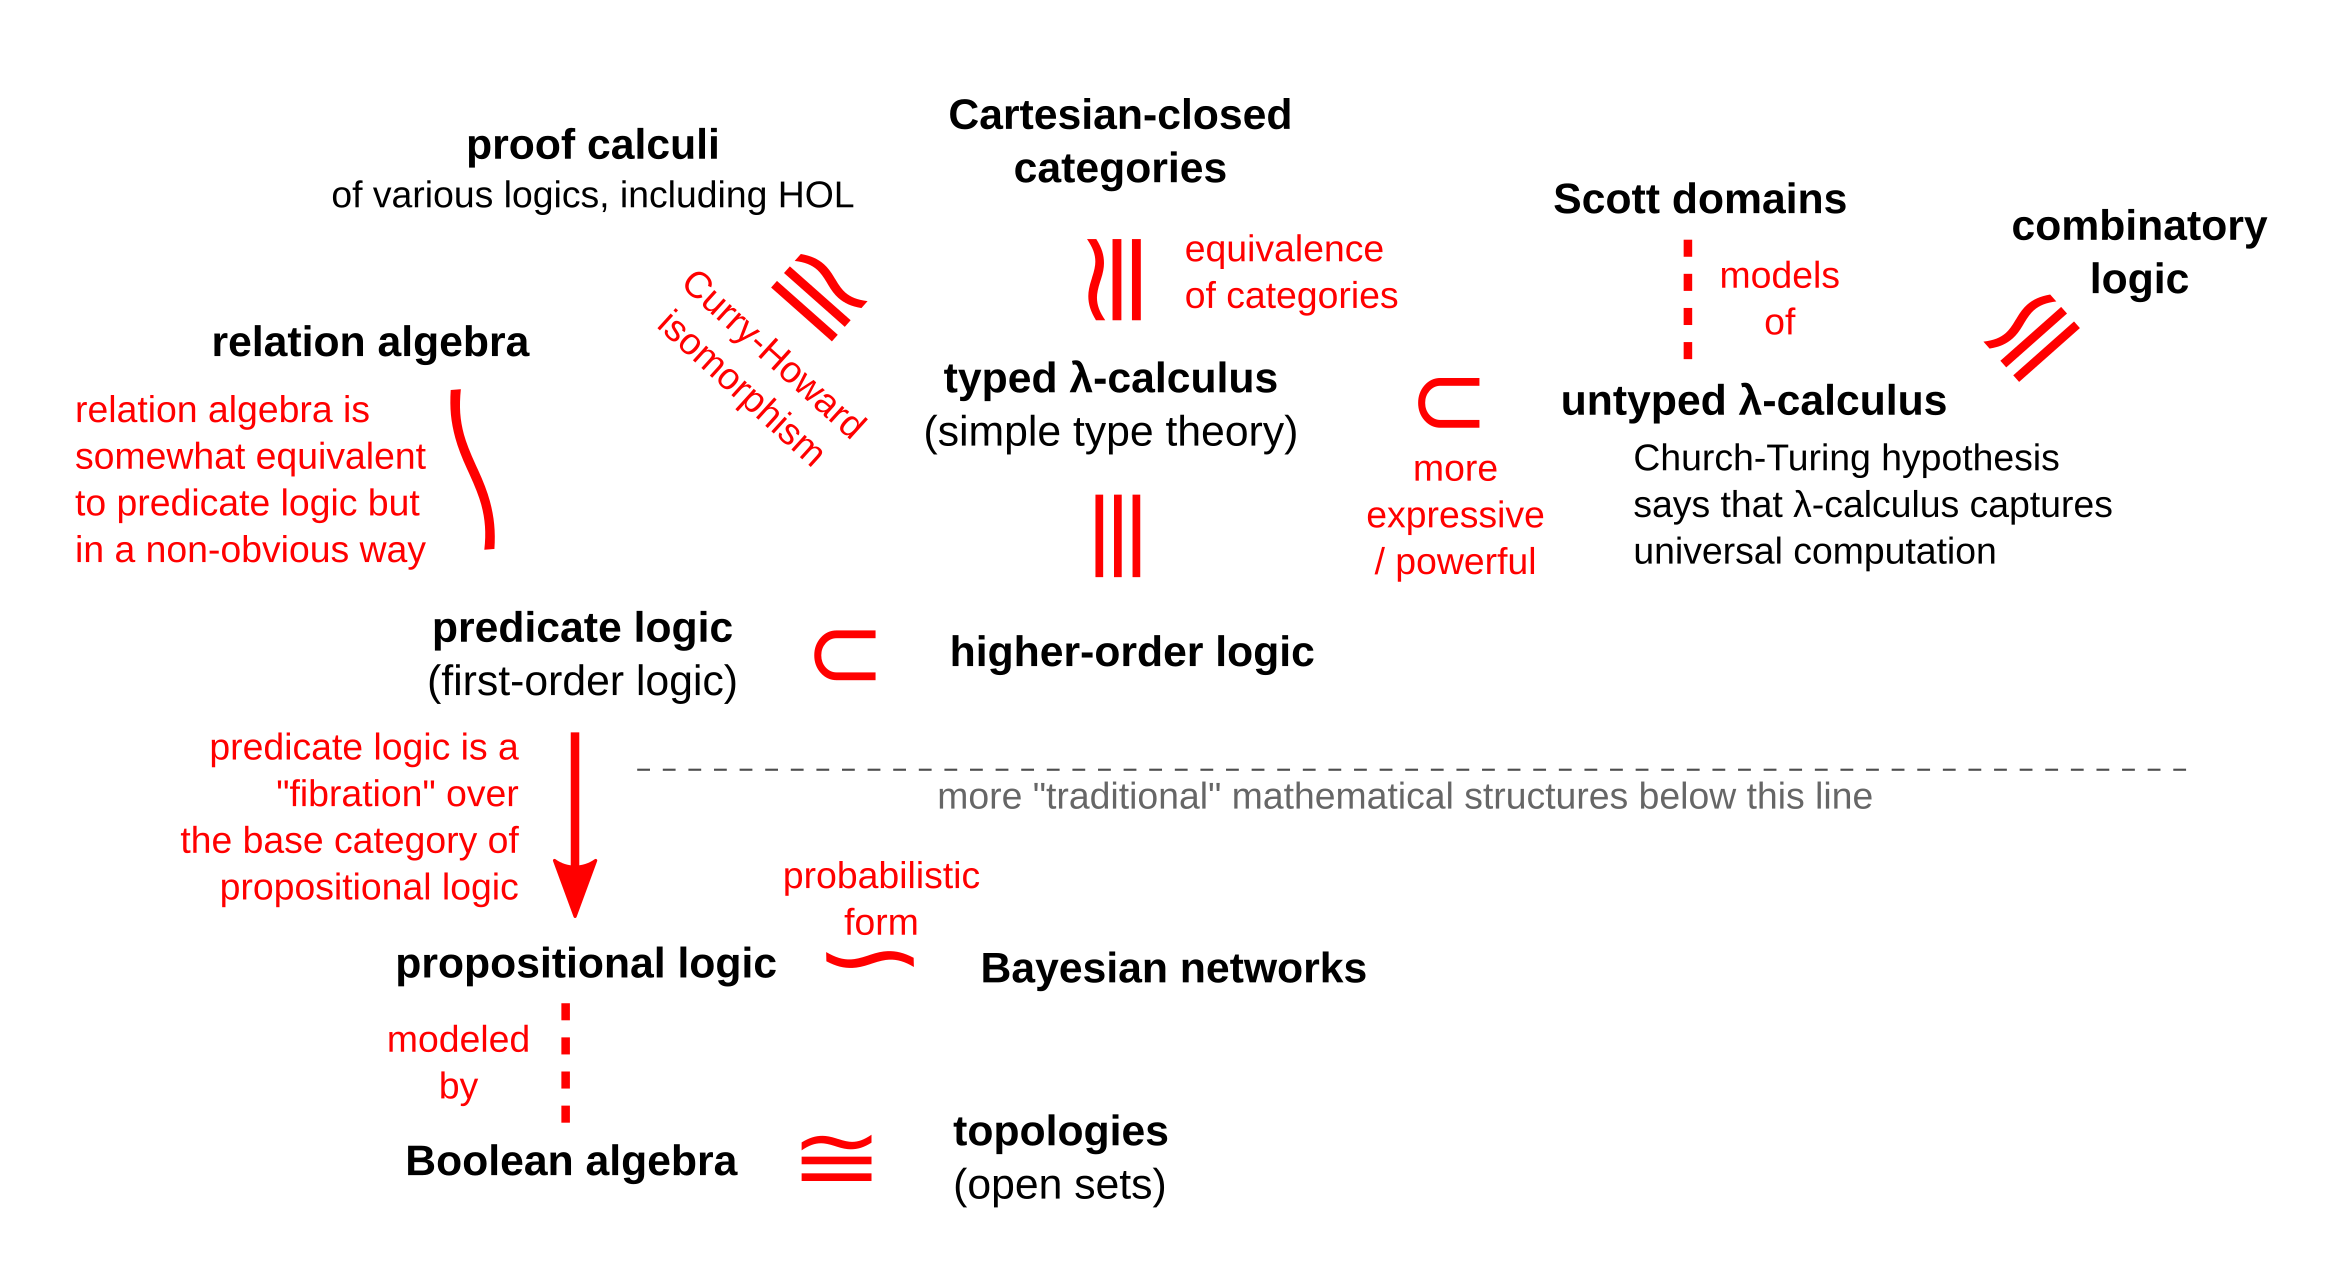
\includegraphics[scale=0.6]{world-of-logical-structures.png}}}
\end{equation}
在我正在写的书中有更详细介绍。

\subsection{A simple logic based on sequence-rewriting}

在本文中,我著重介绍一种最简单的逻辑结构。 

「我爱你」$\neq$「你爱我」(造成这世界很多痛苦):
\begin{equation}
\boxed{世界很多痛苦} \quad a \cdot b \neq b \cdot a
\end{equation}
换句话说,在 sub-propositional level(由概念组成命题的层次),其结构是一个 \textbf{non-commutative} 的东西,这东西或许是 group / semi-group / monoid.

「我爱你 $\wedge$ 你爱我」=「你爱我 $\wedge$ 我爱你」(为方便记忆,找个口号):
\begin{equation}
\boxed{人生不是绝望} \quad A \wedge B = B \wedge A
\end{equation}
换句话说,在 propositional level(命题层次),结构是某个 \textbf{commutative} group / semi-group / monoid.

将这两个层次合起来,得到的是一个 group algebra(或者可以是 non-commutative ring, .... etc),这些是 \textbf{抽象代数} 中最为熟悉的结构,在数学上十分方便。  (暂时我还未考虑 distributive law 是否成立这个问题)

补充一点: 在机器学习中,为了加快学习速度,会引入一些 \textbf{约束},缩小搜寻空间的大小,此谓之 \textbf{inductive bias}.  数学上,搜寻空间通常是一些代数结构,例如 lattice,我们的目的是求原空间的 quotient(商空间),即 mod 掉某 equivalence class,而这 equivalence 可以是某个 symmetry。

再补充一点: 加速学习的方法,还有 \textbf{transfer learning} 和 \textbf{meta-learning}.  其实这二者都是 inductive bias,基本上它们 start with a relatively ``free'' structure,在某些 \textbf{狭窄} 的 domain 上学习,由此学习出来的 bias 当成是 \textbf{长期的} bias。 而我现时的做法是(在抽象代数方面)用人手设计 inductive bias。

TO-DO:  证明这种逻辑的 expressive power is equivalent to first-order logic (or higher-order logic?)  (我个人推测它至少等价於 FOL,这证明或许在某些书里已有)

Proof outline:
\begin{itemize}
	\item FOL terms can be translated as a sum-of-product terms
	\item how to handle $\forall$ and $\exists$ formulas?
	\item every FOL inference step can be realized as sequence-rewriting of such terms
\end{itemize}

\subsubsection{将逻辑分拆成概念(命题)和知识(推导)}

在我设计的这个 representation scheme 里:
\begin{eqnarray}
\label{eqn:logic-knowledge-decomposition}
\mbox{逻辑项 (terms)} & \leftrightsquigarrow & \mbox{代数结构中的元素 (elements)} \nonumber \\
\mbox{逻辑蕴涵 (logical implication)} & \leftrightsquigarrow & \mbox{代数结构之间的 mapping: element $\mapsto$ element}
\end{eqnarray}
换句话说,将逻辑结构分拆成两部分: 元素,和元素之间的 mappings。 

代数元素 = \textbf{逻辑概念} 及其组成的 \textbf{命题}。  Mapping = 由某些命题 $\rightarrow$ 另一些 命题。  换句话说,the set of mappings 代表系统的\textbf{知识} 的全部,它是 人工智能 赖以 思考 的「引擎」,对应於经典 AI 的 ``rules base''。  这些 mappings 交给 deep neural network 学习,因为 deep learning 是现时最强的机器学习方法。 

换句话说,整体策略是:
\begin{itemize}
	\item 将逻辑 \textbf{概念} 和 \textbf{命题} embed 到 vector space 上
	\item 用 deep learning 学习 这些 vectors 之间的 mapping
\end{itemize}

\subsubsection{Implementation with symmetric neural networks}

Architecture 的细节有待 spell out 出来,但其中最关键的似乎是那 commutative 部分: 如何用神经网络处理 commutative(或者可以叫 symmetric)结构?  将神经网络 $\NN$ 记作 $F(\vect{x})$,则我们希望有:
\begin{equation}
F(x,y) = F(y,x)
\end{equation}
$x,y$ 是输入 vector 的 两部分。

如果将第一层 weight matrix 造成 \textbf{左右对称},则 symmetry 很容易满足,但这忽略了更深层的 layers,不算是 ``deep symmetric neural network''。   然而,深层由於有非线性的 sigmoid functions,很难求出满足对称性的 weights 的条件。 换句话说,\uline{单靠设定 神经网络 内部的 weights},很难做到 symmetric NN。

最近我间接读到,Abel 在 1826 年提出了一个 symmetric functional equation 的问题,那篇可能是最早的 semi-group 论文,受此启发:
\begin{equation}
F(x,y) + F(y,x) \quad \mbox{或} \quad F(x,y) \cdot F(y,x)
\end{equation}
等形式都可以是 symmetric functions,其中 $F$ 是任意神经网络。 这解决了关键的一步。

\subsection{Higher-order logic}

如上所述,逻辑形式 的选择有很多可能,包括 $\lambda$-calculus 和 combinatory logic。  和它们比较,我提出的 simple re-writing logic 可能不够 powerful,这一点有待证明。 

重温一下 基本 architecture:
\begin{equation}
\vcenter{\hbox{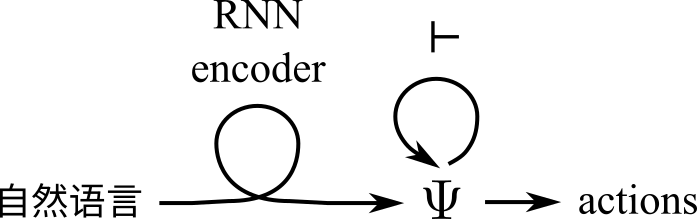
\includegraphics[scale=0.7]{AGI-foundation-3.png}}}
\end{equation}
这里 $\Psi$ 的逻辑形式基本上可以是任何结构。  接下来我们考虑怎样用 $\lambda$-calculus 或 combinatory logic 做 $\Psi$ 的结构....

\subsubsection{$\lambda$-calculus}

基本上,$\lambda$-calculus 是一种关於 \textbf{函数} 的演算法。  它可以表示成一种 monoid,其乘法是 function composition.  但 $\lambda$-calculus 还包含 $\alpha$-, $\beta$-, $\eta$- reduction 的定义,这些法则决定了 \textbf{variable substitutions} 的意义,同时也很麻烦,它们似乎不能被纳入上述 monoid 的定义之中。 

依据我先前 simple logic 的思路,问题是如何基於 $\lambda$-calculus 做到类似 (\ref{eqn:logic-knowledge-decomposition}) 的分拆,但这似乎不是最好的途径,\uline{因为由 $\lambda$-calculus 通往 logic 的最「自然」途径是 Curry-Howard isomorphism}.  根据后者的理论:
\begin{eqnarray}
\lambda\mbox{-terms} &\leftrightsquigarrow& \mbox{proofs} \nonumber \\ 
\mbox{types} &\leftrightsquigarrow& \mbox{propositions}
\end{eqnarray}

按照 Curry-Howard 的思想,问题是如何将 \textbf{神经网络} 引入到这框架中?  例如,将所有 $\lambda$-terms embed 到 vector space 上,然后用神经网络学习 $\lambda$-terms 的演算法,亦即 $\lambda$-calculus.  问题是,为什么觉得 神经网络 能胜任这个任务?  

更重要的是: 釐清在 Curry-Howard 思想下,$\lambda$-calculus 是如何做 \textbf{逻辑推导} 的?   经典 AI 的 knowledge rules 对应於 $\lambda$-calculus 或 Curry-Howard correspondence 里的什么? 

\subsubsection{Combinatory logic}

Combinatory logic 等价於 $\lambda$-calculus,其逻辑化方法应该根据以上的理论。  另方面,或者可以参考 \textbf{illative combinatory logic} 的做法。  (待续)

肖达 \textit{et al}

\begin{comment}
\section{Deep RNN}

The equation for one layer of RNN is:
\begin{equation}
x_{n+1} = \sigmoid (W x + H x)
\end{equation}
\end{comment}

\section*{Acknowledgements}

\bibliographystyle{unsrtnat} % or number or aaai ...
\bibliography{AGI-book}

\end{document}
